\documentclass[11pt]{article}
\usepackage[margin=1in]{geometry}
\usepackage{hyperref}
\usepackage{enumitem}
\usepackage{tikz}
\usetikzlibrary{arrows.meta, positioning}
\setlist{nosep,leftmargin=*}
\title{Rubric-Aware Agentic Proposal Builder with Human-in-the-Loop Critique and Verifiable Revision}
\author{CS NLP Course Project Proposal}
\date{}
\begin{document}
\maketitle
\vspace{-1.4em}

\section*{Abstract}
This project proposes an agentic, rubric-aware system that converts a rough research idea into a complete, citation-grounded research proposal. The system represents proposal requirements as an executable checklist and uses specialized agents for planning, retrieval, drafting, critique, human feedback, and revision. The main hypothesis is that a verifiable revision loop will produce higher required-section coverage, fewer unsupported high-severity claims, stronger citation-link presence, and higher human rubric scores than a single-shot ChatGPT-style drafting baseline. User efficiency will be treated as an optional measured outcome using time-on-task and number of manual edits, not as an assumed benefit. The one-quarter deliverable is a working prototype, evaluation on 12 rough ideas, and a documented release package.

\section*{Keywords}
research proposal generation; agentic AI; rubric-aware evaluation; human-in-the-loop revision; citation grounding; verifiable LLM systems

\section*{Introduction: Motivation, Gap, and Target Context}
CS students writing a first research proposal often know a topic but struggle to express motivation, novelty, methods, risks, and evaluation in a rubric-compliant form. Teaching assistants must then judge not only final prose quality, but also whether claims are supported and whether revisions actually addressed critique findings.

Generic LLM chat systems can produce fluent one-shot drafts, yet in informal use they may omit required sections, blur citations, and provide little audit evidence for how weaknesses were corrected. The target context is a single-student NLP course project over 12 weeks, using an LLM API with a local deterministic fallback for checklist validation and reproducible logs.

\section*{Novelty and Relation to Prior Work}
Retrieval-augmented generation grounds answers in retrieved documents, and ALCE studies citation generation for LLM outputs. Self-Refine and Reflexion show that language agents can improve outputs through iterative feedback, while the uploaded Civio reading note suggests that compliance-oriented writing workflows can become practical tools.

The novelty claim is scoped and verifiable: for the course proposal task, this project will test whether representing the rubric as structured data improves generation and revision compared with a single-shot baseline. The system will operationalize the rubric as checklist items linked to proposal sections, source notes, critique findings, human accept or reject decisions, and revision diffs. Rather than claiming that no other tools support compliance, the evaluation will report which of these traceability features are present in the prototype and absent or manually unavailable in the baseline runs.

\section*{Goal}
The goal is to design, implement, and evaluate a prototype that transforms a rough CS research idea into a proposal while testing improvements in rubric coverage, citation grounding, revision transparency, and user control compared with a single-shot LLM drafting baseline.

\section*{Methods: Agent Workflow}
The system maintains a structured JSON proposal state containing user intent, rubric items, section plans, candidate sources, draft text, critique findings, decisions, and revision history. Figure~\ref{fig:workflow} shows the compact workflow.

\begin{enumerate}
\item \textbf{Intake and requirement extraction.} Inputs are the rough idea, course rubric, and optional references; outputs are normalized checklist items, assumptions, and missing-information questions.
\item \textbf{Planning and retrieval.} A planner maps requirements to proposal sections, while a retrieval agent queries sources such as Semantic Scholar, Crossref, OpenAlex, arXiv, or a curated corpus and stores metadata with snippets.
\item \textbf{Drafting and grounding.} A drafting agent writes concise LaTeX sections and attaches source notes to factual or comparative claims; unsupported claims are marked as assumptions rather than asserted.
\item \textbf{Critique, human decision, and revision.} A rubric critic reports missing sections, weak novelty statements, unsupported claims, and evaluation gaps. The user accepts, rejects, or edits recommendations, and a revision agent updates only linked sections while preserving the audit log.
\item \textbf{Stopping criteria.} The loop stops when all required sections are covered, no high-severity unsupported claims remain, evaluation targets are explicit, or the user reaches a time or iteration limit.
\end{enumerate}

\begin{figure}[t]
\centering
\footnotesize
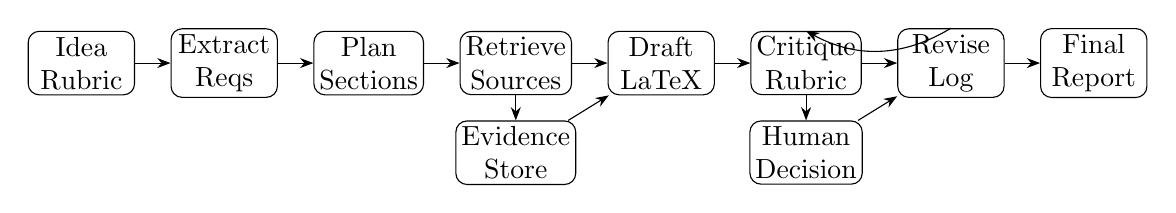
\begin{tikzpicture}[node distance=0.32cm and 0.45cm, box/.style={draw, rounded corners, align=center, minimum width=1.35cm, minimum height=0.52cm, inner sep=2pt}]
\node[box] (idea) {Idea\\Rubric};
\node[box, right=of idea] (req) {Extract\\Reqs};
\node[box, right=of req] (plan) {Plan\\Sections};
\node[box, right=of plan] (ret) {Retrieve\\Sources};
\node[box, right=of ret] (draft) {Draft\\LaTeX};
\node[box, right=of draft] (crit) {Critique\\Rubric};
\node[box, right=of crit] (rev) {Revise\\Log};
\node[box, right=of rev] (final) {Final\\Report};
\node[box, below=of ret] (evid) {Evidence\\Store};
\node[box, below=of crit] (human) {Human\\Decision};
\draw[-{Stealth}] (idea) -- (req);
\draw[-{Stealth}] (req) -- (plan);
\draw[-{Stealth}] (plan) -- (ret);
\draw[-{Stealth}] (ret) -- (draft);
\draw[-{Stealth}] (draft) -- (crit);
\draw[-{Stealth}] (crit) -- (rev);
\draw[-{Stealth}] (rev) -- (final);
\draw[-{Stealth}] (ret) -- (evid);
\draw[-{Stealth}] (evid) -- (draft);
\draw[-{Stealth}] (crit) -- (human);
\draw[-{Stealth}] (human) -- (rev);
\draw[-{Stealth}, bend left=30] (rev.north) to (crit.north);
\end{tikzpicture}
\caption{Rubric-aware proposal generation with evidence storage, human decisions, and a verifiable revision loop.}
\label{fig:workflow}
\end{figure}

\section*{Expected Results and Milestones}
Expected outputs are a prototype that accepts rough ideas and checklists, a rubric-to-section coverage matrix, citation-grounded claim notes, an iterative critique and revision mechanism, and an evaluation report against explicit baselines.
\begin{itemize}
\item Weeks 1--2: finalize rubric, user tasks, metrics, baseline prompt, and annotation guide.
\item Weeks 3--4: design JSON state, agent roles, prompt templates, and audit schema.
\item Weeks 5--6: implement intake, planning, drafting, and LaTeX output validation.
\item Weeks 7--8: add retrieval, source metadata, and claim-source linking.
\item Weeks 9--10: implement rubric critic, revision loop, and human decision interface.
\item Weeks 11--12: run evaluation, analyze failures, prepare demo, documentation, and release notes.
\end{itemize}

\section*{Evaluation}
The study will use 12 rough proposal ideas across three CS domains. Each idea will be run under two primary conditions: \textbf{B1}, a single-shot ChatGPT-style prompt that asks for the full proposal at once using the same idea and rubric; and \textbf{Ours}, the full workflow with extraction, retrieval notes, critique, human decision capture, and one revision pass. If time permits, an ablation without retrieval will test the value of citation grounding separately.

Automatic metrics will be computed for every output: required-section coverage out of 13, with target 13 of 13 for the revised workflow; high-severity unsupported-claim count, with target 0 after one revision; citation-link presence for factual or comparative claims, with target at least 90\%; successful LaTeX compilation, with target 100\%; and audit completeness, measured as the percentage of critique findings linked to a user decision and a revision outcome, with target at least 90\%. Optional user-efficiency metrics are time-on-task and number of manual edits needed to reach a submission-ready proposal.

Human evaluation will ask at least two advanced students, TAs, or expert reviewers to rate novelty, method clarity, evaluation quality, citation grounding, and overall readiness on a 1--5 rubric. The target is mean score $\geq 4.0$ for revised outputs and a positive difference between Ours and B1. The report will include per-metric means, failure cases, and examples where the audit log confirms that a critique item was fixed.

\section*{Risks and Mitigation}
\begin{itemize}
\item \textbf{Hallucinated citations:} require retrieved metadata or mark the claim as an assumption.
\item \textbf{Weak retrieval:} allow curated seed papers and manual source upload.
\item \textbf{Workflow complexity:} keep seven agent stages but expose one user-facing checklist.
\item \textbf{User fatigue:} ask only high-value questions tied to blocked requirements.
\item \textbf{Subjective evaluation:} combine automatic checks, blinded human ratings, and before-after comparisons.
\end{itemize}

\section*{Resources, Tools, and Release Plan}
Resources include an LLM API or local model, Python orchestration, a lightweight web or notebook interface, JSON storage, LaTeX validation, and retrieval from Semantic Scholar, Crossref, OpenAlex, arXiv, institutional databases, or a curated paper corpus. The release will include a prototype demo, prompt and workflow templates, anonymized examples, evaluation scripts, and open-source orchestration code where API and corpus licenses allow.

\section*{References and Assumptions}
\begin{enumerate}
\item Patrick Lewis et al. ``Retrieval-Augmented Generation for Knowledge-Intensive NLP Tasks.'' NeurIPS, 2020.
\item Tianyu Gao et al. ``ALCE: Enabling Large Language Models to Generate Text with Citations.'' EMNLP, 2023.
\item Aman Madaan et al. ``Self-Refine: Iterative Refinement with Self-Feedback.'' NeurIPS, 2023.
\item Noah Shinn et al. ``Reflexion: Language Agents with Verbal Reinforcement Learning.'' NeurIPS, 2023.
\item Uploaded course materials and reading note: proposal requirements, grading rubric, and Civio compliance-workflow note. Assumption: these materials define the target rubric and reviewer expectations.
\end{enumerate}

\end{document}